\section{Curva de Fronteira de Produção}
A curva ou também chamada de fronteira, é um dos mais básicos e importantes conceitos da economia. Ele descreve todas as combinações de produtos que podem ser produzidos caso os meios de produção sejam utilizados. Essa curva mostra a quantidade máxima que pode ser produzida de um dado bem sendo limitado pelo seus finitos recursos e tecnologia. Todos os valores fora da curva são impossíveis por conta de suas limitações.\par
É possível através da análise desta curva podemos concluir que devemos abrir mão da produção de certos bens em detrimento de outros. Para se acessar pontos fora da curva é necessário se melhorar os meios de produção, esses por sua vez estão ligados a tecnologia.\par
\begin{figure}[!ht]
    \centering
    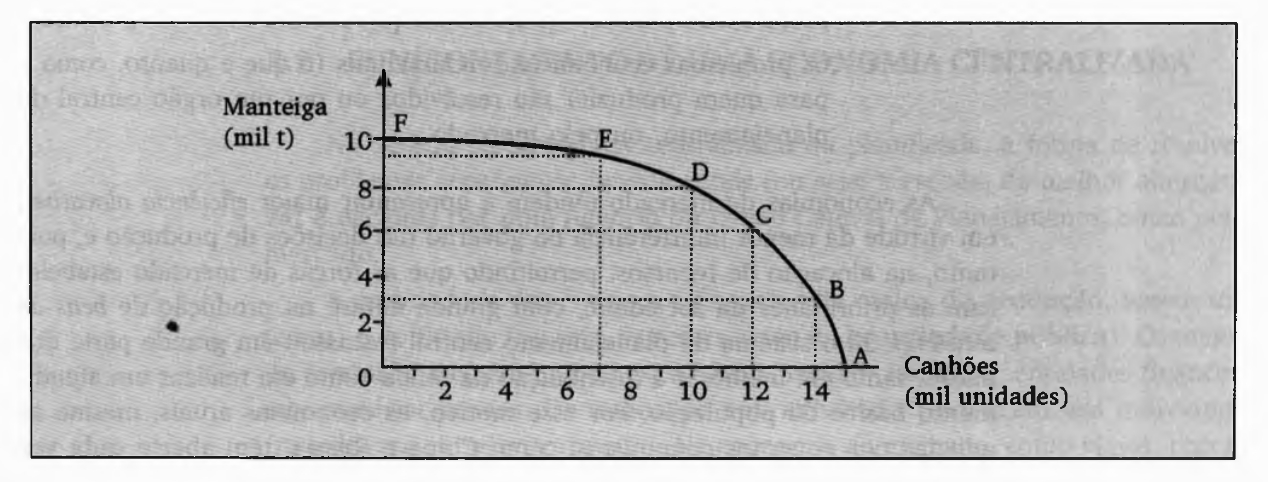
\includegraphics[width=\textwidth]{curva.jpg}
    \caption{Curva de Possibilidades de Produção}\citep{emm}
    \label{fig:cpp}
\end{figure}
\subsection{Custo de oportunidade}
Dado uma quantidade de recursos, quanto esses utilizados de forma eficiente é possível se produzir uma quantidade de bens, para se aumentar a produção desse bem, é preciso reduzir a produção de um outro bem.\par
A esse exemplo é dado o nome de Custo de Oportunidade, um conceito intrínseco da economia, onde, para se produzir mais de um bem A é necessário que se reduza a produção de um bem B. Ao se mover na curva de fronteira de produção, é possível ver a quantidade de um bem B que se deve abrir mão para produzir mais de um bem A. O custo de oportunidade de um bem também é chamado de custo real, já que ele representa a quantidade de um bem que deve ser sacrificada para a produção de outro.\par
\clearpage